\chapter{Movement Duration Minimizes Variability and Effort Concurrently: An Optimal Control Model}
\label{cha:ocmd}
\outline{1}{Movement Duration Minimizes Variability and Effort Concurrently}

\section{Introduction}
Our previous work (Chapter \ref{cha:md}, published \cite{Wang2016}) demonstrated through experimental data that 
(1) in arm reaching movement without visual feedback, an intermediate movement duration minimizes endpoint variability; 
(2) the durations of reaching movements chosen by our subjects were longer than the durations minimizing endpoint variance. 
\cite{Wang2016} proposed that 
(1) two kinds of execution noise, Constant (CN) and Signal-Dependent Noise (SDN), lead to endpoint variability respectively at long and short movement durations, hence the joint effects of CN and SDN result in an intermediate movement duration that minimizes endpoint variability;
(2) effort is also minimized together with endpoint variability, which drives subjects to choose a duration that is longer that the duration minimizing endpoint variability.

Hypothesis (1) expands previous works on effects of execution noise in motor planning and control.
\cite{Harris1998, Harris2006} used SDN and minimum endpoint variance to account for reaching movement planning and kinematics. 
However, their model cannot distinguish minimizing endpoint variability due to SDN from minimizing effort, because formulation of effort often\footnote{For example, when effort is defined as the integral of squared torque or motor commands} leads to equivalent mathematical expressions as endpoint variance \cite{Wang2016, OSullivan2009}. 
Moreover, since minimizing variability due to SDN slows down movement, they failed to explain subjects, given a specific task, do not move slower than they do to achieve smaller endpoint variability.
Since movements with longer duration have larger endpoint variability with the presence of CN \cite{Todorov2005}, our hypotheses consider CN as another component of execution noise, such that minimizing variability would yield a compromise between SDN and CN, leading to a specific movement duration. 
The level of CN estimated in \cite{VanBeers2004} to account for endpoint distributions was comparable with the level of SDN, showing that CN as an execution noise cannot be ignored.

Optimal control theory assumes that movements can be understood as the solution of an optimization process.
The cost function of this optimization process is generally composed of two parts: one encodes the goal of the movement; the other penalizes some inherent feature of the movement \cite{Diedrichsen2010}. 
The first part can be formularized as the endpoint variance \cite{Harris1998}, or the endpoint error \cite{Todorov2005}; 
the second part can be based on the integrated jerk \cite{Flash1985}, integrated torque change \cite{Uno1989}, or integrated squared motor commands \cite{Todorov2002} (which was what we used in this work). 
To our knowledge, The relationship between movement duration and the two parts of the cost function has not been examined systematically and thoroughly.
Our hypothesis (2) provides insights on the distinct role of movement variability (first part of the cost function) and effort (second part of the cost function) for determining the duration of a movement.

We tested our hypotheses in computer simulations using stochastic open-loop optimal control \cite{Todorov2005} model with CN and SDN as execution noise.  
Although $\sigma_{\text{SDN}}$ and $\sigma_{\text{CN}}$ (see equation \ref{eqn:cnsdn} have previously been estimated \cite{VanBeers2004}, these estimates were based on inverse dynamics control of a simulated arm with a viscosity parameter that was estimated at rest from restoring forces to small perturbations \cite{Gomi1998}. 
However, the amount of viscosity during movements is presumably substantially smaller during movement than at rest \cite{Burdet2013}. 
In addition, we found in simulations (results not shown) that viscosity has a profound effect on the distribution of endpoints.  
We therefore re-estimated $\sigma_{\text{SDN}}$ and $\sigma_{\text{CN}}$ as well as a free viscosity parameter by fitting an optimal open-loop controller to endpoint reaching data in Chapter \ref{cha:md}.

We then used these parameters to simulate reaching movements, and investigated endpoint variability and effort of movement with different durations.
%Our results reveal distinct roles of CN, SDN, and effort in planning movements.

\section{Methods}
To test our hypothesis, we built an open-loop stochastic optimal control model with both SDN and CN, estimated the levels of CN and SDN through the matching of the model with data in Chapter \ref{cha:md}, and simulated endpoint distributions and effort of movement with different movement durations.

\subsection{Open-loop Stochastic Optimal Control Model}
The reaching movement is simulated with a planar arm with a shoulder and an elbow, whose joint angles are represented by $\bm{q} = (q_1, q_2)^T$, controlled by the open-loop stochastic optimal controller. 
The forward and inverse kinematics are formulated as in \cite{VanBeers2004}, and the dynamics equation is

\begin{equation} \label{maindynamics}
	\ddot{\bm{q}} = \bm{M}(\bm{q})^{-1} (\bm{\tau} - \bm{C}(\bm{q}, \dot{\bm{q}}) - \bm{B}\dot{\bm{q}})
\end{equation}

where $\bm{M}(\bm{q})$ is the inertia matrix, $\bm{C}(\bm{q}, \dot{\bm{q}})$ accounts for the centrifugal force and the Coriolis effect, and $\bm{B}$ is the viscosity matrix, which we assume to be a diagonal matrix with a single value $b$ on the diagonal. $b$ is a free parameter as discussed above. 
See Supplemental Material \ref{app:kindyn} for matrices definitions and parameter values.

We use a second-order linear filter as the muscle model (as in \cite{VanBeers2004}) which receives motor commands and gives torques over joints:

\begin{equation}
	\bm{u} = t_et_a\ddot{\bm{\tau}} + (t_e+t_a)\dot{\bm{\tau}} +\bm{\tau}
\end{equation}

where $\bm{u}$ is the motor command, $t_e = 30$ ms, $t_a = 40$ ms are time constants representing excitation and activation respectively \cite{VanderHelm2000}. 

The motor command $\bm{u}$ is corrupted with signal-dependent noise and constant noise:

\begin{equation}\label{eqn:cnsdn}
u_t \rightarrow (1 + \epsilon\sigma_{\text{SDN}}) u_t + \xi\sigma_{\text{CN}}
\end{equation}

where $\epsilon$ and $\xi$ are random variables from the normal Gaussian distribution.
$\sigma_{\text{CN}}$ and $\sigma_{\text{SDN}}$ represent the levels of noise.

To circumvent the difficulty of solving a nonlinear optimal control problem, we discretized and linearized the kinematics and dynamics equations with 10 ms time step interval around an approximated solution (as in \cite{Li2004}, details shown in Supplemental Material \ref{ocformulation}), giving rise to a linear-quadratic problem with the following cost to minimize:

\begin{equation}\label{eqn:cost}
V = \bm{s}_T^T\bm{Q}_T\bm{s}_T + \sum_{t=1}^T\bm{u}_t^T\bm{Ru}_t
\end{equation}

where $\bm{s_t}$ is the state vector. 
$\bm{Q}$ is arranged in such a way that the first term represents the square of endpoint error in hand space (Supplemental Material \ref{app:cost}). 
$\bm{R}$ is a diagonal matrix with a single value $w_r$ on the diagonal.
$w_r$ is a free parameter.
The second term, the integral of squared motor commands, is assumed to be the effort being considered in the process of determining movement duration. 

\subsection{Endpoint Distribution from Gaussian Execution Noise}

As shown in equation \ref{eqn:cnsdn}, the execution noise (CN and SDN) are assumed independent and Gaussian. 
The endpoint distribution due to execution noise is generally not Gaussian due to nonlinearity of the kinematics and dynamics. 
Through linearization of the system, we essentially used Gaussian as an approximation of the actual endpoint distribution. 
This approximation makes the algorithm much more efficient (thanks to the covariance propagation equation, see Supplemental Material \ref{app:covarProp}), than simulating large number of trials and calculating statistics over the endpoints (seen in \cite{VanBeers2004,Guigon2008}).
In order to make sure this approximation is appropriate, we compared the distribution from the linearized system to the original nonlinear system. As shown in figure \ref{fig:linearizeddistributionapprox}, the Gaussian distributions given by the linearized system (the blue 95\% confidence ellipse) are good approximations of the actual distributions of the original nonlinear system (the 2-dimension histogram, from 6000 simulated endpoints).

\begin{figure}
	\centering
	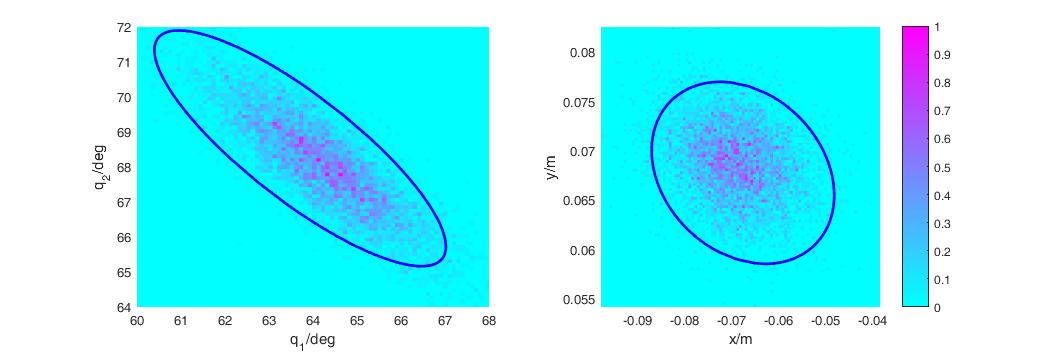
\includegraphics[width=\linewidth]{figures/linearizedDistributionApprox}
	\caption[Endpoint distributions of linearized system approximate the original]{Endpoint distributions of linearized system approximate the original. On the left is the distribution of joint angles at the endpoint position; on the right is the distribution of endpoints in task space. The blue 95\% confidence ellipses are distributions of linearized system; the 2-dimension histogram are distributions of the original system.}
	\label{fig:linearizeddistributionapprox}
\end{figure}

\subsection{Estimation of SDN and CN in Reaching Movements}
Although $\sigma_{\text{SDN}}$ and $\sigma_{\text{CN}}$ (see equation \ref{eqn:cnsdn}) have previously been estimated in \cite{VanBeers2004}, these estimates were based on inverse dynamics control of a simulated arm with a viscosity parameter that was estimated at rest from restoring forces to small perturbations \cite{Gomi1998}. 
However, the amount of viscosity during movements is presumably substantially smaller during movement than at rest \cite{Burdet2013}. 
In addition, we found in simulations (Supplemental Material \ref{app:oc}) that viscosity has a profound effect on the distribution of endpoints.  
We therefore re-estimated $\sigma_{\text{SDN}}$ and $\sigma_{\text{CN}}$ with viscosity as a free parameter by fitting an optimal open-loop controller to reaching data described in Chapter \ref{cha:md}.

We picked the $\sigma_{\text{SDN}}$ and $\sigma_{\text{CN}}$ values that minimize the following fitting error function:

\begin{equation}
\label{eqn:fiterror}
\sum_{t}\sum_{c} (\text{TE}_{\text{data},t,c} - \text{TE}_{\text{sim},t,c})^2
\end{equation}

where $t$ and $c$ are indexes for target and condition, and TE stands for Total Error defined as 

\begin{equation}
\text{TE}_{\text{data}} = \frac1N\sum_n \left( (x - x^*)^2 + (y - y^*)^2 \right) 
\end{equation}

where $n$ is index for trials;

\begin{equation}
\text{TE}_{\text{sim}} = (\bar{x} - x^*)^2 + (\bar{y} - y^*)^2 + \text{tr}(\bm{P})
\end{equation}

where $(\bar{x},\bar{y})$ and $\bm{P}$ are the first (mean) and second (covariance matrix) central moment of the simulated endpoint distribution. 
The expressions of TE for data and simulation are different because $\text{TE}_{\text{data}}$ is calculated from actual endpoint data, whereas $\text{TE}_{\text{sim}}$ is calculated from the first and second moment of endpoint distribution.
We used \textsf{patternsearch} in Matlab to determine $\sigma_{\text{CN}}$ and $\sigma_{\text{SDN}}$ as well as viscosity parameter $ b $ that minimize the fitting error function \ref{eqn:fiterror}. 
In addition, we systematically varied $ w_r $ from $ 10^{-7} $ to 〖$ 10^{-5} $, but found that it had very little effect on both endpoint distributions and estimation of other three free parameters (at most 5\%). We therefore set $ w_r $ = $ 2\times 10^{-6} $ because larger values lead to inability of reaching to the target and smaller values decrease effect of effort minimization in movement generation. 
		
We found that for simulated movement that is longer than 1 second, the endpoint variability is very sensitive to CN.
We therefore assume $\sigma_{\text{CN}}$ depends on movement durations, but $\sigma_{\text{SDN}}$ is constant. [need rational and citation] 

With the estimated  $\sigma_{\text{CN}}$ and $\sigma_{\text{SDN}}$ as well as viscosity parameter $ b $, we simulated reaching movements to both targets with different movement duration.

\section{Results}

\subsection{Estimation of SDN and CN in Reaching Movements}

The minimization of the fitting error function yielded the following noise and viscosity parameters: $\sigma_{\text{SDN}} = 0.298$ (unit-less), $\sigma_{\text{CN}}$(fast, medium, preferred, slow) = (0.010, 0.037, 0.035, 0.031)(\si{N.m}), and $b=0.110$ (\si{kg.m^2/s}). 
Note that our estimation of viscosity is significantly lower than \cite{VanBeers2004}. 

We interpolate $\sigma_{\text{CN}}$ as a function of movement duration using piecewise cubic Hermite interpolation \cite{Fritsch1980}, shown in figure \ref{fig:interpcn}.

\begin{figure}
	\centering
	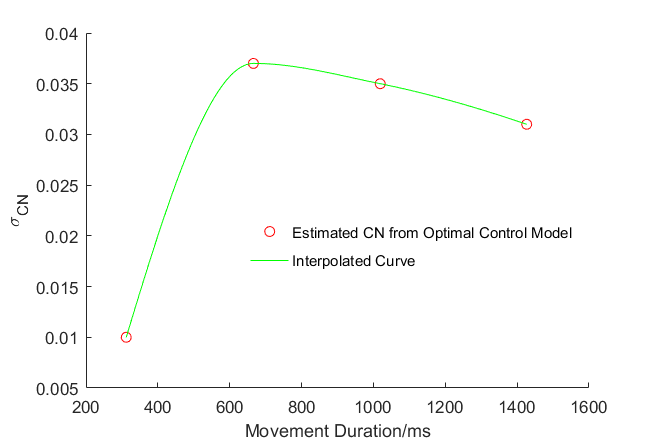
\includegraphics[width=0.75\linewidth]{figures/interpCN}
	\caption[Interpolation of $\sigma_{\text{CN}}$]{The Interpolation of $\sigma_{\text{CN}}$ against movement duration using piecewise cubic Hermite interpolation. The constant noise level is low at fast movement, and increases with movement duration, until it reaches a plateau.}
	\label{fig:interpcn}
\end{figure}

The model with estimated noise and viscosity parameters produces a Movement Duration - Total Error relationship that is very close to the data, shown in figure \ref{fig:total-error}.

\begin{figure}
	\centering
	\includegraphics[width=\linewidth]{"figures/total error"}
	\caption[Model with estimated parameters reproduces U curve relationship between Movement Duration and Total Error]{Model with estimated parameters reproduces U curve relationship between Movement Duration and Total Error. The model has 6 free parameters: four $\sigma_{\text{CN}}$ values for four movement durations,  $\sigma_{\text{SDN}}$, viscosity $ b $.}
	\label{fig:total-error}
\end{figure}



\subsection{Simulation of Cost vs. Movement Duration}

For both the \ang{45} and the \ang{135} targets, the stochastic optimal control model with parameters estimated above produced a U-shape relationship between total error and movement duration (Figure \ref{fig:variability---cost---minimum-shift}). 
The total error reached a minimum at an intermediate movement duration (approximately 600 ms for both targets), and increased either for faster or slower movements. 

The total cost (equation \ref{eqn:cost}) also exhibited a U-shape characteristic. 
For the left target, the total cost curve reached the minimum at about 1000 ms, very close to the average movement duration (1053 ms) that the subjects chose at the preferred condition. 
However, for the right target, the total cost curve reached the minimum at a movement duration only a little longer than the movement duration that minimizes the total error, not enough to the average movement duration (about 1000 ms) that the subjects chose at the preferred condition.
The difference stems from the larger effort required for a movement to the target at \ang{135} (which involves both shoulder and elbow rotation) than the target at \ang{45} (which involves roughly to an elbow rotation), as shown by the yellow curve in figure \ref{fig:variability---cost---minimum-shift}. 


\begin{figure}
	\centering
	\includegraphics[width=\linewidth]{"figures/variability - cost - minimum shift"}
	\caption[Simulation of Cost vs. Movement Duration Curve]{Simulation of Cost vs. Movement Duration Curve. The minimum of cost curve is at longer movement duration than the minimum of error curve, for both left and right target. The minimm of cost curve for the left target is at the "preferred" movement duration that the subjects choose in preferred condition (see Chapter \ref{cha:md}); However, for the right target, the minimum of cost curve is not at the "preferred" movement duration.}
	\label{fig:variability---cost---minimum-shift}
\end{figure}


\section{Discussion}
%If a task does not specifically (explicitely) have a varibility limit, then minimizing endpoint variance with SDN or minimizing effort inevitably leads to infinitely long movement duration. Therefore, additional mechanism is needed to reduce the movement duration. [Shadmehr 2010, 2016] proposes that the movement duration pose a discount of reward of the goal, which is called the "Cost of Time". Although Although this hypothesis has its base on physiological studies (Johnson  Bickel, 2002), but the discounting time constant is in the range of days or months. Whether discounting works within seconds remains to be confirmed. Another mechanism to reduce movement duration is to consider Constant Noise (CN). In Van Beers work, it has been shown that the effect of CN is not negligible ... and [authors] shows that CN in optimal control model, leads to larger variability at longer duration. Thus minimizing endpoint variability due to both signal-dependent and constant noise would yield a minimum that could determine movement duration. Correspondingly, our first hypothesis is that the CNS chooses intermediate reaching movement durations to minimize endpoint variability in the face of signal-dependent and constant noise.

It has long been known that the duration of arm movements has an effect on endpoint variability  \cite{Woodworth1899, Fitts1954}, but the relationship had not been systematically characterized. 
Our modeling results showed that, in coherence with data \ref{cha:md}, an intermediate movement duration minimizes total endpoint error. 
Such intermediate movement duration was predicted by the presence of SDN and CN in the motor command and was previously found in saccadic movements \cite{VanBeers2008}, but had not been observed in reaching movements. 
In addition, the model showed that the minimization of endpoint variability and effort yields longer movement duration than minimizing only endpoint variability.
This behavior of the model, for a subset of movement direction (the \ang{135} target), is coherent with data in Chapter \ref{cha:md}; however, the movement duration to the \ang{45} target was not well accounted for by the model. The effort required for the \ang{45} target, compared to the \ang{135} target, is very small, because the movement involves mostly only the elbow joint rotation. 
What's more, the use of squared motor command makes the effort decreases cubically with movement duration \cite{Shadmehr2016}, rendering the effect of effort very small to have an impact on the cost curve \ref{fig:variability---cost---minimum-shift}. 
We plan to use an optimal control model with an effort term in the cost function defined as the integral of absolute value of motor commands (which decreases linearly with movement duration).
It is reasonable to expect the effect of effort not so small at longer movement with a L1 norm effort term.
Nevertheless, our model supports the notion that effort is a determinant of movement planning in the context of SDN and CN on the motor command. 
Future work should aim at validating our estimate of effort e.g. via quantification of metabolic costs, e.g. \cite{Huang2012}.

Although minimum motor variability and minimum effort models appear conceptually different, \cite{OSullivan2009} pointed out that they are tightly related when only SDN is included: endpoint variance, which increases with SDN, corresponds to the effort deployed during the movement \cite{OSullivan2009}. 
Therefore, when considering either of these two factors, an additional term has to be considered in the cost minimized by the CNS to prevent selection of the slowest possible movements. 
It has for instance been proposed that subjects select such as the longest movement duration for which the hand is expected to land in the target with high probability \cite{Hoff1994,Harris1998,Harris2006}, or use temporal discounting of reward \cite{Shadmehr2010, Rigoux2012, Haith2012}. Our model does not require such additional factor to explain our data.
Instead, using a combination of SDN and CN, with the standard deviations of these two noise sources directly identified from reaching data in the first experiment, the model provides a parsimonious mechanistic explanation for the overall pattern of errors across the fast, medium, and slow movement durations.  
Future work will be needed to dissociate the effects of constant noise and discounting, in both movements with and without vision.

A further contribution of our study is the re-estimation of the contributions of $\sigma_{\text{SDN}}$ and $\sigma_{\text{CN}}$ in reaching movements. 
$\sigma_{\text{SDN}}$ has been estimated according to the force produced during isometric muscle contraction \cite{Jones2002, Slifkin1999} in saccadic movements, and in pointing movements without visual feedback \cite{VanBeers2004}. $\sigma_{\text{CN}}$ has been estimated in saccadic movements \cite{VanBeers2008} and pointing movements without visual feedback using a feedforward control model \cite{VanBeers2004}. 
Here, re-estimation of the noise parameter in arm reaching movements by setting viscosity as a free parameter yielded greater $\sigma_{\text{SDN}}$ compared to $\sigma_{\text{N}}$ than previously thought. We found $\sigma_{\text{SDN}}$ = 0.298 (unit-less) and $\sigma_{\text{CN}}$ $\sim$ 0.01-0.04 (N m), compared to $\sigma_{\text{SDN}}$ = 0.103 and $\sigma_{\text{CN}}$= 0.185 (N m) in \cite{VanBeers2004}. 

Van Beers et al. added to CN and SDN a third noise source called “temporal noise”, which was not needed in our model to account for the data. 
Note, however, that proprioceptive feedback was not taken into account both in van Beers’s and in our model, notably because the effect of such feedback on movements seem small for movements at normal speed (see e.g. Figure 4 in \cite{Franklin2007}). 
However, for slower movements the effect of such feedback on endpoint error may become more important – thus, the effect of such feedback would be to decrease the slope of the rightward portion of the U curves in simulations of Figure \ref{fig:variability---cost---minimum-shift}. 
As a result, the preferred movement times and the movement times that minimize variance in the model would be longer and, therefore, more in line with those of the experimental results. 
However, this would not modify the result that, in the context of SDN and CN, effort determines movement duration.


\section{Supplemental Material on Stochastic Control Modeling}
\label{app:oc}

\subsection{Kinematics and Dynamics}
\label{app:kindyn}
The forward kinematics, inverse kinematics and dynamics of this two-link arm model are widely used in the literature (e.g \cite{VanBeers2004}):

\begin{equation}
\bm{r} =\left(\begin{matrix} x\\y \end{matrix}\right) % = \text{FK}(\bm{q}) 
= \left[ \begin{matrix}  l_1\cos{q_1} + l_2\cos{(q_1+q_2)} \\ l_1\sin{q_1} + l_2\sin{(q_1+q_2)}  \end{matrix} \right]
\end{equation}
\begin{equation}
\begin{split}
& q_2 = \arccos{\left(\frac{r^2-l_1^2-l_2^2}{2l_1l_2}\right)} \\
& q_1 = \arctan{\left( \frac{y}{x} \right)} - \arctan{\left(\frac{l_2\sin{q_2}}{l_1+l_2\cos q_2 }\right)}
\end{split}
\end{equation}
\begin{equation} \label{dynamics}
\ddot{\bm{q}} = \bm{M}(\bm{q})^{-1} (\bm{\tau} - \bm{C}(\bm{q}, \dot{\bm{q}}) - \bm{B}\dot{\bm{q}})
\end{equation}

where $\bm{M}(\bm{q})$ is the inertia matrix, $\bm{C}(\bm{q}, \dot{\bm{q}})$ accounts for the centrifugal force and the Coriolis effect, and $\bm{B}$ is the viscosity matrix:

\begin{equation}
\bm{M} = \left( \begin{matrix} a_1 + 2a_2\cos\theta_2  &  a_3 + a_2 \cos\theta_2 \\
a_3 + a_2 \cos\theta_2   &  a_3
\end{matrix}\right)
\end{equation}
\begin{equation}
\bm{C} = \left( \begin{matrix} -\dot{\theta_2}(2\dot{\theta_1}+\dot{\theta_2}) \\
\dot{\theta_1}^2	\end{matrix} \right)
a_2\sin{\theta_2}
\end{equation}
\begin{equation}
\bm{B} = \left( \begin{matrix} b_1  & 0 \\ 0 & b_2 \end{matrix} \right)
\end{equation}
\begin{equation}
a_1 = I_1 + I_2 + m_2 l_1^2
\end{equation}
\begin{equation}
a_2 = m_2 l_1 s_2
\end{equation}
\begin{equation}
a_3 = I_2
\end{equation}

Arm length $\bm{l} = (l_1, l_2)^T$ = (30cm, 33cm), arm mass $m_i =$ (1.4kg, 1kg), $s_i=$ (11cm, 16cm) is the distance from the joint center to the center of the mass for link i , and $I_i$ = ($0.025\text{kgm}^2, 0.045\text{kgm}^2$) is the moment of inertia.

We use a second-order linear filter as the muscle model (as in Van Beers) which receives motor commands and gives torques over joints:

\begin{equation}
\bm{u} = t_et_a\ddot{\bm{\tau}} + (t_e+t_a)\dot{\bm{\tau}} +\bm{\tau}
\end{equation}

where $\bm{u}$ is the motor command, $t_e$, $t_a$ are time constants for excitation and activation respectively. 
The second order filter can be divided into two first order filter, respectively corresponding to excitation and activation:

\begin{equation}
\begin{split}
& \bm{u} = t_e \dot{\bm{e}} + \bm{e} \\
& \bm{e} = t_a \dot{\bm{\tau}} + \bm{\tau}
\end{split}
\end{equation}

All variables in \textbf{bold} letters (such as $\bm{e}$) have two components corresponding to shoulder and elbow.

The motor command $\bm{u}$ is corrupted with signal-dependent noise and constant noise:

\begin{equation}
u_t \rightarrow (1 + \epsilon\sigma_{\text{SDN}}) u_t + \xi\sigma_{\text{CN}}
\end{equation}

where $\epsilon$ and $\xi$ are random variables from the normal Gaussian distribution.
$\sigma_{\text{CN}}$ and $\sigma_{\text{SDN}}$ represent the levels of the noise.

\subsection{Optimal Control Formulation}
\label{ocformulation}

We choose Linear Quadratic Regulator (LQR) \cite{Li2004} to formulate the optimal control problem. Since the plant is nonlinear, a generalized LQR called iterative LQR (iLQR) is adopted here.

\subsubsection{LQR with signal dependent noise}
Standard LQR deals with independent Gaussian noise. To generalize to signal dependent noise (SDN) is quite straightforward. I conclude the result here.

Given the dynamics (linear) and cost function (sum of cost rate, quadratic), the problem is to get motor command $\bm{u}_t$ such that the cost function is minimized.
\begin{equation}\label{optimprob}
\begin{split}
\text{dynamics:~~} & \bm{x}_{t+1} = \bm{Ax}_t + \bm{Bu}_t + \bm{\xi}_t + \epsilon_t\bm{Cu}_t \\
\text{cost rate:~~} & \bm{x}_t^T\bm{Q}_t\bm{x}_t + \bm{u}_t^T\bm{Ru}_t
\end{split}
\end{equation}
$\bm{\xi}$ is the constant noise, $\epsilon\bm{Cu}$ is the signal dependent noise; $\bm{\xi}$ and $\epsilon$ are random variables. Specifically, $\epsilon$ is set to have unit standard deviation. Here I include only one source of SDN. To add more, simply add similar terms in the solution.

The solution is given by the following control policy:
\begin{equation}
\bm{u} = -(\bm{R}+(\bm{B+C})^T\bm{V}_{t+1}(\bm{B+C}) )^{-1} \bm{B}^T\bm{V}_{t+1}\bm{Ax}
\end{equation}
where $\bm{V}_t$ is the cost-to-go matrix 
\begin{equation}
\bm{V}_t = \bm{Q}_t + \bm{A}^T\bm{V}_{t+1}\bm{A} - \bm{A}^T\bm{V}_{t+1}\bm{B}(\bm{R} + (\bm{B+C})^T\bm{V}_{t+1}(\bm{B+C}))^{-1}\bm{B}^T\bm{V}_{t+1}\bm{A}
\end{equation}

\subsubsection{Linearization}
To formulate the model in the form of LQR, a linearization is required. First is to discretize all time-dependent variables :
\begin{equation}
\begin{split}
\bm{q}_{t+1} &= \bm{q}_{t} + \dot{\bm{q}_{t}} \Delta t \\
\dot{\bm{q}}_{t+1} &= \dot{\bm{q}}_{t} + \ddot{\bm{q}}_{t} \Delta t \\
\bm{\tau}_{t+1} &= \bm{\tau}_{t} + \dot{\bm{\tau}_{t}} \Delta t \\
\bm{e}_{t+1} &= \bm{e}_{t} + \dot{\bm{e}_{t}} \Delta t \\
\end{split}
\end{equation}
The only nonlinear part is $\ddot{\bm{q}}_t$, in another word, $\dot{\bm{q}}_{t+1}$ is a nonlinear function of $\bm{q}_t$, $\dot{\bm{q}}_t$, ${\bm{\tau}}_t$, ${\bm{e}}_t$. Define the state vector 
\begin{equation}
\bm{x}_t=\left[ \begin{matrix}\bm{q}_t \\ \dot{\bm{q}}_t \\ \bm{\tau}_t \\ \bm{e}_t \end{matrix} \right]
\end{equation}
The linearized dynamics appears to be
\begin{equation}
\bm{x}_{t+1} - \tilde{\bm{x}}_{t+1} = \bm{A}_t (\bm{x}_t - \tilde{\bm{x}}_{t}) + \bm{B}(\bm{u}_t - \tilde{\bm{u}}_t)
\end{equation}
where $\tilde{\bm{x}}_t$ and $\tilde{\bm{u}}_t$ is any pair set of state and command, and matrix $\bm{A}_t$, as following, is evaluated at $\tilde{\bm{x}}_t$:
\begin{equation}
\bm{A}_t = \left[\begin{matrix}
1 & 0 & \Delta t & 0  & 0 & 0 & 0 & 0 \\
0 & 1 & 0 &\Delta t   & 0 & 0 & 0 & 0 \\
0 & \frac{\partial{\dot{q}_1^{t+1}}}{\partial{q_2^t}} & \frac{\partial{\dot{q}_1^{t+1}}}{\partial{\dot{q_1}^t}} & \frac{\partial{\dot{q}_1^{t+1}}}{\partial{\dot{q_2}^t}} & \frac{\partial{\dot{q}_1^{t+1}}}{\partial{\tau_1^t}} & \frac{\partial{\dot{q}_1^{t+1}}}{\partial{\tau_2^t}}& 0& 0 \\
0 & \frac{\partial{\dot{q}_2^{t+1}}}{\partial{q_2^t}} & \frac{\partial{\dot{q}_2^{t+1}}}{\partial{\dot{q_1}^t}} & \frac{\partial{\dot{q}_2^{t+1}}}{\partial{\dot{q_2}^t}} & \frac{\partial{\dot{q}_2^{t+1}}}{\partial{\tau_1^t}} & \frac{\partial{\dot{q}_2^{t+1}}}{\partial{\tau_2^t}}& 0& 0 \\
0 & 0 & 0 & 0   &   1-\frac{\Delta t}{t_a} & 0 & \frac{\Delta t}{t_a} & 0 \\
0 & 0 & 0 & 0   &   0 & 1-\frac{\Delta t}{t_a} & 0 & \frac{\Delta t}{t_a} \\
0 & 0 & 0 & 0   &   0 & 0 & 1-\frac{\Delta t}{t_e} & 0 \\
0 & 0 & 0 & 0   &   0 & 0 & 0 & 1-\frac{\Delta t}{t_e} \\
\end{matrix}\right]
\end{equation}
\begin{equation}
\bm{B} = \left[\begin{matrix}
0 & 0 \\
0 & 0 \\
0 & 0 \\
0 & 0 \\
0 & 0 \\
0 & 0 \\
\frac{\Delta t}{t_e} & 0 \\
0 & \frac{\Delta t}{t_e} 
\end{matrix}\right]
\end{equation}
Now the dynamics equation can be written as
\begin{equation}\label{dynam}
\begin{split}
\bm{x}_{t+1} &= \bm{A}_t \bm{x}_t + \bm{B}\bm{u}_t + \bm{c}_t \\
\bm{c}_t &= \tilde{\bm{x}}_{t+1} - \bm{A}_t\tilde{\bm{x}}_{t} - \bm{B}\tilde{\bm{u}}_t
\end{split}
\end{equation}

\subsubsection{Cost Function}
\label{app:cost}
Usually there are two terms in the cost function; one is the cost for motor command $\bm{u}$, the other is for endpoint error $\bm{x} - \bm{x}^*$. To make both of them representable in quadratic form, $\bm{x}^*$ has to be imbedded into the state vector, so the new state vector is now defined as
\begin{equation}
\bm{x}_t=\left[ \begin{matrix}\bm{q}_t \\ \dot{\bm{q}}_t \\ \bm{\tau}_t \\ \bm{e}_t \\
\bm{q}^* \\ \dot{\bm{q}}^*
\end{matrix} \right]
\end{equation}
To make a quadratic cost function, the matrix $\bm{Q}$ must take the following form:
\begin{equation}
\bm{Q} = 
\left( \begin{matrix}
\bm{I}_{4\times4} \\
\bm{0}_{4\times4} \\
\bm{-I}_{4\times4} 
\end{matrix} \right)
\bm{J}^T
\left( \begin{matrix}
w_p &&&\\
&w_p&& \\
&&w_v&\\
&&&w_v 
\end{matrix} \right)
\bm{J}
\left( \begin{matrix}
\bm{I}_{4\times4} &
\bm{0}_{4\times4} &
\bm{-I}_{4\times4} 
\end{matrix} \right)
\end{equation}
where $w_p$ and $w_v$ are weights for position error and velocity error respectively, and $\bm{J}$ is the Jacobian matrix. The matrices $\bm{A}$ and $\bm{B}$ in dynamics equation also change:
\begin{equation}
\begin{split}
\bm{A} & \leftarrow \left( \begin{matrix}
\bm{A} \\
&\bm{I}_{4\times4} \\
\end{matrix} \right) \\
\bm{B} & \leftarrow \left( \begin{matrix}
\bm{B} \\
\bm{0}_{4\times2} \\
\end{matrix} \right)
\end{split}
\end{equation}
In conclusion, the result of linearization is the following LQR problem:
\begin{equation}\label{linlqr}
\begin{split}
\text{dynamics:~~}\bm{x}_{t+1} =& \bm{A}_t \bm{x}_t + \bm{B}\bm{u}_t + \bm{c}_t \\
(\text{where~~~}\bm{c}_t = & \tilde{\bm{x}}_{t+1} - \bm{A}_t\tilde{\bm{x}}_{t} - \bm{B}\tilde{\bm{u}}_t) \\
\text{cost:~~~~~~~~~~~} & \bm{x}_T^T\bm{Q}_T\bm{x}_T + \sum_{t=1}^T\bm{u}_t^T\bm{Ru}_t \\
\end{split}
\end{equation}

\subsubsection{Iterative LQR}
The solution to equation \ref{linlqr} is not the solution to the original nonlinear problem, since it is just a linear approximation around $\tilde{\bm{x}}_t$ and $\tilde{\bm{u}}_t$. However, the solution can be taken as a new start point, and so on. When the iteration converges, the solution to equation \ref{linlqr} is $\tilde{\bm{u}}_t$ itself.

\subsubsection{Covariance Matrix Propagation}\label{app:covarProp}
Once we get the optimal solution $\tilde{\bm{u}}$ from iterative LQR, we can plug it back into equation \ref{linlqr} (the same as the dynamics equation \ref{dynam}) to get the optimal trajectory. We can also turn on SDN in a form that is consistent with equation \ref{optimprob}, and/ or any form of constant noise, to simulate arm movement with motor/ state noise. The statistics of multiple simulations then can be compared with experiment data.

Many works look at the characters of endpoint distributions of arm reaching movement \cite{VanBeers2004, Guigon2008}. Instead of running repetitively the simulations, there is another way to get the endpoint distribution, namely to calculate the covariance matrix of the state vector after each time step. Let us consider equation \ref{dynam} with motor command $\bm{u}_t$ corrupted with constant noise (CN) and signal dependent noise (SDN). That is,
\begin{equation}
u_t \rightarrow (1 + \epsilon\sigma_{\text{SDN}}) u_t + \xi\sigma_{\text{CN}}
\end{equation}
where $\epsilon$ and $\xi$ are random variables with normal distribution, $\sigma$ represents the standard deviation of the motor noise. We also assume that the noise of different components of $\bm{u}$ are independent from each other, though they share the standard deviation. We have,
\begin{equation}
E[\bm{u}_t\bm{u}_t^T] = 
\left(\begin{matrix}
\sigma_{\text{CN}}^2 + 		\sigma_{\text{SDN}}^2 u_{1t}^2   &  0 \\
0  &   \sigma_{\text{CN}}^2 + 		\sigma_{\text{SDN}}^2 u_{2t}^2   \\
\end{matrix}\right)  \equiv \bm{Q}_t
\end{equation}
I omit the mean of the variables for simplicity. Apply to the dynamics equation \ref{dynam}, Let $\bm{P}_t = E[\bm{x}_{t}\bm{x}_{t}^T]$ we have
\begin{equation}
\bm{P}_{t+1} = \bm{A}_t \bm{P}_t\bm{A}_t^T + \bm{B}\bm{Q}_t\bm{B}^T
\end{equation}

\subsection{Results}\label{results}
\subsubsection{Effects of Viscosity}
In \cite{VanBeers2004}, The viscosity matrix $\bm{B}$ in equation \ref{dynamics} is set to be diagonal with a value of 0.8 Nms/rad:
\begin{equation}
\bm{B} = 
\left(\begin{matrix}
0.8 & 0 \\
0 & 0.8 \\
\end{matrix}\right)
\end{equation}
Here I compare simulation results with \cite{VanBeers2004} value and a value of zero.

For a movement to a 90 degree target, simulation with high viscosity value gives S-shaped trajectory and asymmetric velocity profile  (figure \ref{fig:0.8}), whereas simulation with zero viscosity gives bell shaped velocity profile (figure \ref{fig 0.0}).
\begin{figure}[h]
	\centering
	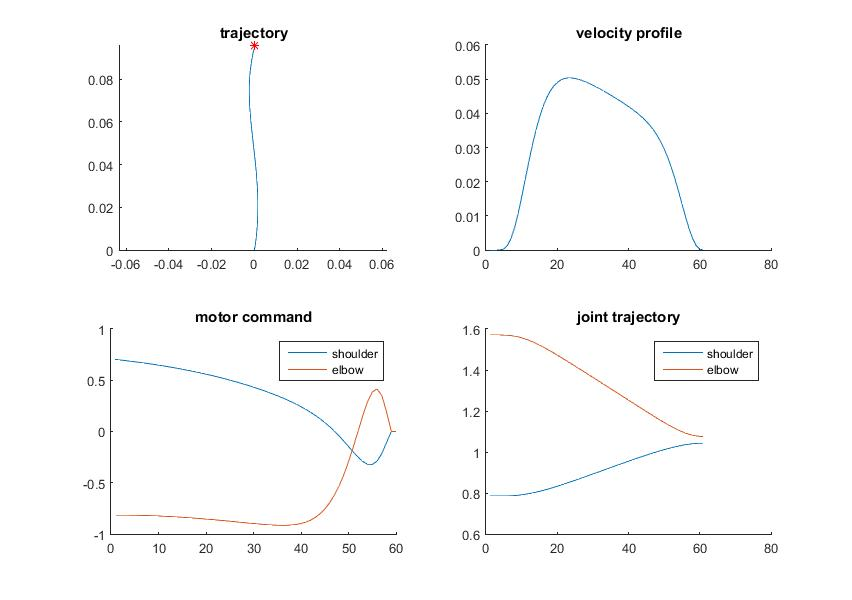
\includegraphics[width=\textwidth]{up8} 
	\caption{simulation result with high viscosity value}
	\label{fig:0.8}
\end{figure}
\begin{figure}[h]
	\centering
	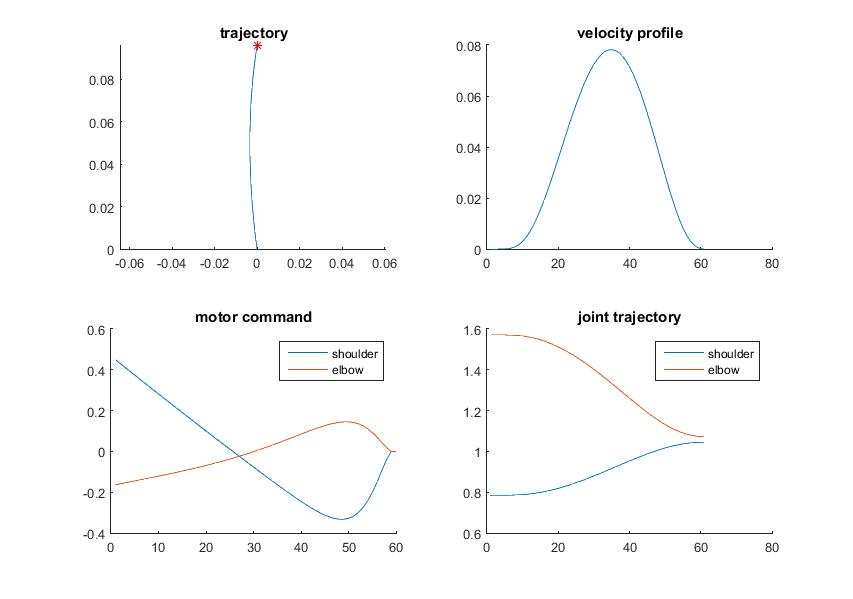
\includegraphics[width=\textwidth]{up0}
	\caption{simulation result with zero viscosity value}
	\label{fig 0.0}
\end{figure}



